\begin{figure}[tbp]\centering
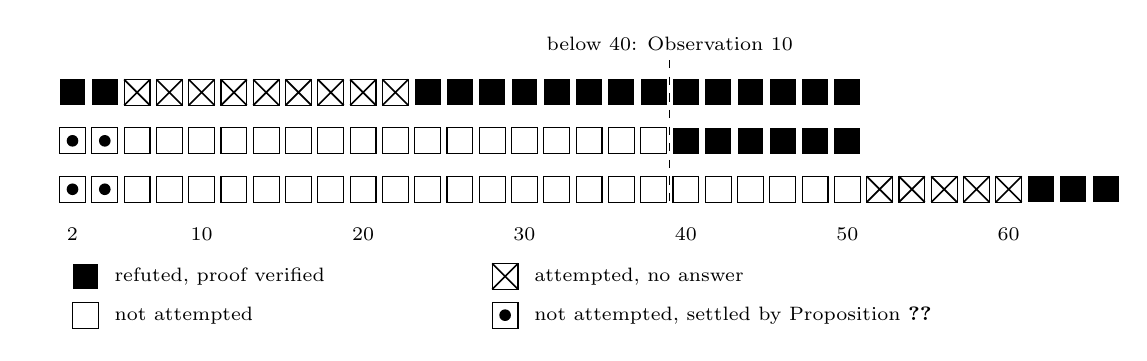
\begin{tikzpicture}[solid, x=0.41cm, y=0.41cm, font=\scriptsize]
\node[anchor=east] at (0.2,0.0) {$\Ga$};
\path[fill=black] (0.6,-0.4) rectangle (1.4,0.4);
\path[fill=black] (1.6,-0.4) rectangle (2.4,0.4);
\path[draw, line width=0.4pt] (2.6,-0.4) rectangle (3.4,0.4);
\draw[line width=0.6pt] (2.6,-0.4) -- (3.4,0.4) (2.6,0.4) -- (3.4,-0.4);
\path[draw, line width=0.4pt] (3.6,-0.4) rectangle (4.4,0.4);
\draw[line width=0.6pt] (3.6,-0.4) -- (4.4,0.4) (3.6,0.4) -- (4.4,-0.4);
\path[draw, line width=0.4pt] (4.6,-0.4) rectangle (5.4,0.4);
\draw[line width=0.6pt] (4.6,-0.4) -- (5.4,0.4) (4.6,0.4) -- (5.4,-0.4);
\path[draw, line width=0.4pt] (5.6,-0.4) rectangle (6.4,0.4);
\draw[line width=0.6pt] (5.6,-0.4) -- (6.4,0.4) (5.6,0.4) -- (6.4,-0.4);
\path[draw, line width=0.4pt] (6.6,-0.4) rectangle (7.4,0.4);
\draw[line width=0.6pt] (6.6,-0.4) -- (7.4,0.4) (6.6,0.4) -- (7.4,-0.4);
\path[draw, line width=0.4pt] (7.6,-0.4) rectangle (8.4,0.4);
\draw[line width=0.6pt] (7.6,-0.4) -- (8.4,0.4) (7.6,0.4) -- (8.4,-0.4);
\path[draw, line width=0.4pt] (8.6,-0.4) rectangle (9.4,0.4);
\draw[line width=0.6pt] (8.6,-0.4) -- (9.4,0.4) (8.6,0.4) -- (9.4,-0.4);
\path[draw, line width=0.4pt] (9.6,-0.4) rectangle (10.4,0.4);
\draw[line width=0.6pt] (9.6,-0.4) -- (10.4,0.4) (9.6,0.4) -- (10.4,-0.4);
\path[draw, line width=0.4pt] (10.6,-0.4) rectangle (11.4,0.4);
\draw[line width=0.6pt] (10.6,-0.4) -- (11.4,0.4) (10.6,0.4) -- (11.4,-0.4);
\path[fill=black] (11.6,-0.4) rectangle (12.4,0.4);
\path[fill=black] (12.6,-0.4) rectangle (13.4,0.4);
\path[fill=black] (13.6,-0.4) rectangle (14.4,0.4);
\path[fill=black] (14.6,-0.4) rectangle (15.4,0.4);
\path[fill=black] (15.6,-0.4) rectangle (16.4,0.4);
\path[fill=black] (16.6,-0.4) rectangle (17.4,0.4);
\path[fill=black] (17.6,-0.4) rectangle (18.4,0.4);
\path[fill=black] (18.6,-0.4) rectangle (19.4,0.4);
\path[fill=black] (19.6,-0.4) rectangle (20.4,0.4);
\path[fill=black] (20.6,-0.4) rectangle (21.4,0.4);
\path[fill=black] (21.6,-0.4) rectangle (22.4,0.4);
\path[fill=black] (22.6,-0.4) rectangle (23.4,0.4);
\path[fill=black] (23.6,-0.4) rectangle (24.4,0.4);
\path[fill=black] (24.6,-0.4) rectangle (25.4,0.4);
\node[anchor=east] at (0.2,-1.5) {$\Gb$};
\path[draw, line width=0.4pt] (0.6,-1.9) rectangle (1.4,-1.1);
\fill (1.0,-1.5) circle (0.18);
\path[draw, line width=0.4pt] (1.6,-1.9) rectangle (2.4,-1.1);
\fill (2.0,-1.5) circle (0.18);
\path[draw, line width=0.4pt] (2.6,-1.9) rectangle (3.4,-1.1);
\path[draw, line width=0.4pt] (3.6,-1.9) rectangle (4.4,-1.1);
\path[draw, line width=0.4pt] (4.6,-1.9) rectangle (5.4,-1.1);
\path[draw, line width=0.4pt] (5.6,-1.9) rectangle (6.4,-1.1);
\path[draw, line width=0.4pt] (6.6,-1.9) rectangle (7.4,-1.1);
\path[draw, line width=0.4pt] (7.6,-1.9) rectangle (8.4,-1.1);
\path[draw, line width=0.4pt] (8.6,-1.9) rectangle (9.4,-1.1);
\path[draw, line width=0.4pt] (9.6,-1.9) rectangle (10.4,-1.1);
\path[draw, line width=0.4pt] (10.6,-1.9) rectangle (11.4,-1.1);
\path[draw, line width=0.4pt] (11.6,-1.9) rectangle (12.4,-1.1);
\path[draw, line width=0.4pt] (12.6,-1.9) rectangle (13.4,-1.1);
\path[draw, line width=0.4pt] (13.6,-1.9) rectangle (14.4,-1.1);
\path[draw, line width=0.4pt] (14.6,-1.9) rectangle (15.4,-1.1);
\path[draw, line width=0.4pt] (15.6,-1.9) rectangle (16.4,-1.1);
\path[draw, line width=0.4pt] (16.6,-1.9) rectangle (17.4,-1.1);
\path[draw, line width=0.4pt] (17.6,-1.9) rectangle (18.4,-1.1);
\path[draw, line width=0.4pt] (18.6,-1.9) rectangle (19.4,-1.1);
\path[fill=black] (19.6,-1.9) rectangle (20.4,-1.1);
\path[fill=black] (20.6,-1.9) rectangle (21.4,-1.1);
\path[fill=black] (21.6,-1.9) rectangle (22.4,-1.1);
\path[fill=black] (22.6,-1.9) rectangle (23.4,-1.1);
\path[fill=black] (23.6,-1.9) rectangle (24.4,-1.1);
\path[fill=black] (24.6,-1.9) rectangle (25.4,-1.1);
\node[anchor=east] at (0.2,-3.0) {$\Gsix$};
\path[draw, line width=0.4pt] (0.6,-3.4) rectangle (1.4,-2.6);
\fill (1.0,-3.0) circle (0.18);
\path[draw, line width=0.4pt] (1.6,-3.4) rectangle (2.4,-2.6);
\fill (2.0,-3.0) circle (0.18);
\path[draw, line width=0.4pt] (2.6,-3.4) rectangle (3.4,-2.6);
\path[draw, line width=0.4pt] (3.6,-3.4) rectangle (4.4,-2.6);
\path[draw, line width=0.4pt] (4.6,-3.4) rectangle (5.4,-2.6);
\path[draw, line width=0.4pt] (5.6,-3.4) rectangle (6.4,-2.6);
\path[draw, line width=0.4pt] (6.6,-3.4) rectangle (7.4,-2.6);
\path[draw, line width=0.4pt] (7.6,-3.4) rectangle (8.4,-2.6);
\path[draw, line width=0.4pt] (8.6,-3.4) rectangle (9.4,-2.6);
\path[draw, line width=0.4pt] (9.6,-3.4) rectangle (10.4,-2.6);
\path[draw, line width=0.4pt] (10.6,-3.4) rectangle (11.4,-2.6);
\path[draw, line width=0.4pt] (11.6,-3.4) rectangle (12.4,-2.6);
\path[draw, line width=0.4pt] (12.6,-3.4) rectangle (13.4,-2.6);
\path[draw, line width=0.4pt] (13.6,-3.4) rectangle (14.4,-2.6);
\path[draw, line width=0.4pt] (14.6,-3.4) rectangle (15.4,-2.6);
\path[draw, line width=0.4pt] (15.6,-3.4) rectangle (16.4,-2.6);
\path[draw, line width=0.4pt] (16.6,-3.4) rectangle (17.4,-2.6);
\path[draw, line width=0.4pt] (17.6,-3.4) rectangle (18.4,-2.6);
\path[draw, line width=0.4pt] (18.6,-3.4) rectangle (19.4,-2.6);
\path[draw, line width=0.4pt] (19.6,-3.4) rectangle (20.4,-2.6);
\path[draw, line width=0.4pt] (20.6,-3.4) rectangle (21.4,-2.6);
\path[draw, line width=0.4pt] (21.6,-3.4) rectangle (22.4,-2.6);
\path[draw, line width=0.4pt] (22.6,-3.4) rectangle (23.4,-2.6);
\path[draw, line width=0.4pt] (23.6,-3.4) rectangle (24.4,-2.6);
\path[draw, line width=0.4pt] (24.6,-3.4) rectangle (25.4,-2.6);
\path[draw, line width=0.4pt] (25.6,-3.4) rectangle (26.4,-2.6);
\draw[line width=0.6pt] (25.6,-3.4) -- (26.4,-2.6) (25.6,-2.6) -- (26.4,-3.4);
\path[draw, line width=0.4pt] (26.6,-3.4) rectangle (27.4,-2.6);
\draw[line width=0.6pt] (26.6,-3.4) -- (27.4,-2.6) (26.6,-2.6) -- (27.4,-3.4);
\path[draw, line width=0.4pt] (27.6,-3.4) rectangle (28.4,-2.6);
\draw[line width=0.6pt] (27.6,-3.4) -- (28.4,-2.6) (27.6,-2.6) -- (28.4,-3.4);
\path[draw, line width=0.4pt] (28.6,-3.4) rectangle (29.4,-2.6);
\draw[line width=0.6pt] (28.6,-3.4) -- (29.4,-2.6) (28.6,-2.6) -- (29.4,-3.4);
\path[draw, line width=0.4pt] (29.6,-3.4) rectangle (30.4,-2.6);
\draw[line width=0.6pt] (29.6,-3.4) -- (30.4,-2.6) (29.6,-2.6) -- (30.4,-3.4);
\path[fill=black] (30.6,-3.4) rectangle (31.4,-2.6);
\path[fill=black] (31.6,-3.4) rectangle (32.4,-2.6);
\path[fill=black] (32.6,-3.4) rectangle (33.4,-2.6);
\node[anchor=north] at (1.0,-3.9) {2};
\node[anchor=north] at (5.0,-3.9) {10};
\node[anchor=north] at (10.0,-3.9) {20};
\node[anchor=north] at (15.0,-3.9) {30};
\node[anchor=north] at (20.0,-3.9) {40};
\node[anchor=north] at (25.0,-3.9) {50};
\node[anchor=north] at (30.0,-3.9) {60};
\draw[dashed, line width=0.5pt] (19.5,1) -- (19.5,-3.5);
\node[anchor=south] at (19.5,1) {below 40: Observation~10};
\path[fill=black] (1,-6.1) rectangle (1.8,-5.3);
\node[anchor=west] at (2,-5.699999999999999) {refuted, proof verified};
\path[draw, line width=0.4pt] (14,-6.1) rectangle (14.8,-5.3);
\draw[line width=0.6pt] (14,-6.1) -- (14.8,-5.3) (14,-5.3) -- (14.8,-6.1);
\node[anchor=west] at (15,-5.699999999999999) {attempted, no answer};
\path[draw, line width=0.4pt] (1,-7.3) rectangle (1.8,-6.5);
\node[anchor=west] at (2,-6.8999999999999995) {not attempted};
\path[draw, line width=0.4pt] (14,-7.3) rectangle (14.8,-6.5);
\fill (14.4,-6.8999999999999995) circle (0.18);
\node[anchor=west] at (15,-6.8999999999999995) {not attempted, settled by Proposition~\ref{prop:small}};
\end{tikzpicture}
\caption{Status of every even target order $k$ below the order of the graph, one cell per order from 2 (left) to $n-2$, for the three graphs of the sweep. The dashed line marks the bound of the cited observation, below which a smaller counterexample is excluded without computation. The cell $k=52$ of the 68-vertex graph is a run stopped before any answer.}\label{fig:map}
\end{figure}
